\documentclass[10pt,a4paper]{article}

\ifdefined\XeTeXversion
  % Tectonic/XeLaTeX branch: use the bundled Unicode face below.
\else
  % Conventional pdfLaTeX users can compile the same source with their local
  % Latin Modern installation.
  \usepackage[utf8]{inputenc}
  \usepackage[T1]{fontenc}
  \usepackage{lmodern}
\fi

\usepackage[a4paper,margin=2.6cm,headheight=15pt]{geometry}
\usepackage{graphicx}
\usepackage{tikz}
\usetikzlibrary{arrows.meta,calc,fit,positioning,shapes.geometric}
\usepackage{enumitem}
\usepackage{xcolor}
\usepackage{listings}
\usepackage{fancyhdr}
\usepackage{lastpage}
\usepackage{hyperref}

% Localize the few structural labels without loading a language package that is
% not present in the offline runtime.
\renewcommand{\figurename}{Figura}

\ifdefined\XeTeXversion
% Use the bundled Unicode font directly so the document also compiles in the
% offline Tectonic runtime used for this deliverable. The same face is mapped
% to the few NFSS shapes needed by headings, listings and body text.
\DeclareFontFamily{TU}{reportfont}{\hyphenchar\font=`\-}
\DeclareFontShape{TU}{reportfont}{m}{n}{<-> "[lmroman10-regular.otf]"}{}
\DeclareFontShape{TU}{reportfont}{m}{it}{<-> "[lmroman10-regular.otf]"}{}
\DeclareFontShape{TU}{reportfont}{m}{sl}{<-> "[lmroman10-regular.otf]"}{}
\DeclareFontShape{TU}{reportfont}{m}{sc}{<-> "[lmroman10-regular.otf]"}{}
\DeclareFontShape{TU}{reportfont}{bx}{n}{<-> "[lmroman10-regular.otf]"}{}
\DeclareFontShape{TU}{reportfont}{bx}{it}{<-> "[lmroman10-regular.otf]"}{}
\renewcommand{\rmdefault}{reportfont}
\renewcommand{\sfdefault}{reportfont}
\renewcommand{\ttdefault}{reportfont}
\AtBeginDocument{\fontencoding{TU}\fontfamily{reportfont}\selectfont}
% A few legacy package macros still request OT1; map those fallbacks to the
% same bundled Unicode face instead of unavailable Type1 metrics.
\DeclareFontFamily{OT1}{cmr}{\hyphenchar\font=`\-}
\DeclareFontShape{OT1}{cmr}{m}{n}{<-> "[lmroman10-regular.otf]"}{}
\DeclareFontShape{OT1}{cmr}{m}{it}{<-> "[lmroman10-regular.otf]"}{}
\DeclareFontShape{OT1}{cmr}{bx}{n}{<-> "[lmroman10-regular.otf]"}{}
\DeclareFontShape{OT1}{cmr}{bx}{it}{<-> "[lmroman10-regular.otf]"}{}
\DeclareFontFamily{OT1}{cmss}{\hyphenchar\font=`\-}
\DeclareFontShape{OT1}{cmss}{m}{n}{<-> "[lmroman10-regular.otf]"}{}
\DeclareFontShape{OT1}{cmss}{bx}{n}{<-> "[lmroman10-regular.otf]"}{}
\DeclareFontFamily{OT1}{cmtt}{\hyphenchar\font=`\-}
\DeclareFontShape{OT1}{cmtt}{m}{n}{<-> "[lmroman10-regular.otf]"}{}
% TikZ and a few table macros use TeX's math families internally for dimensions.
% They are mapped to the same local face to keep the build self-contained.
\DeclareFontShape{OML}{cmm}{m}{it}{<-> "[lmroman10-regular.otf]"}{}
\DeclareFontShape{OMS}{cmsy}{m}{n}{<-> "[lmroman10-regular.otf]"}{}
\DeclareFontShape{OMX}{cmex}{m}{n}{<-> "[lmroman10-regular.otf]"}{}
\fi

\definecolor{navy}{HTML}{12304A}
\definecolor{teal}{HTML}{087E8B}
\definecolor{orange}{HTML}{E76F51}
\definecolor{ink}{HTML}{27313A}
\definecolor{softgray}{HTML}{F3F5F7}
\definecolor{linegray}{HTML}{D6DDE3}
\definecolor{codegreen}{HTML}{2F6F4E}

\hypersetup{
  colorlinks=true,
  linkcolor=navy,
  urlcolor=teal,
  citecolor=navy,
  pdftitle={Informe de avance 3: integración física y línea base E2E},
  pdfauthor={Proyecto de monitoreo vehicular}
}

\setlength{\parindent}{0pt}
\setlength{\parskip}{0.55em}
\setlist{itemsep=0.25em,topsep=0.35em}
\renewcommand{\arraystretch}{1.18}
\newcommand{\code}[1]{\texttt{\small #1}}
\newcommand{\repo}[1]{\href{https://github.com/}{\code{#1}}}

\lstset{
  basicstyle=\ttfamily\footnotesize,
  backgroundcolor=\color{softgray},
  frame=single,
  rulecolor=\color{linegray},
  framerule=0.4pt,
  breaklines=true,
  columns=fullflexible,
  keepspaces=true,
  showstringspaces=false,
  commentstyle=\color{codegreen},
  keywordstyle=\color{navy}\bfseries
}

\pagestyle{fancy}
\fancyhf{}
\fancyhead[L]{\small Informe de avance 3}
\fancyhead[R]{\small Integración física y E2E}
\fancyfoot[C]{\small \thepage\ de \pageref{LastPage}}
\renewcommand{\headrulewidth}{0.4pt}
\renewcommand{\footrulewidth}{0pt}

\begin{document}

\pagenumbering{arabic}

\section*{Resumen}

Este informe documenta el tercer avance del proyecto: la conexión de una placa
ESP32 real con el backend de monitoreo mediante WiFi, NTP, HiveMQ Cloud y MQTT
sobre TLS. El objetivo de esta etapa fue reemplazar la incertidumbre de una
integración únicamente simulada por una línea base física reproducible, sin
confundir esa línea base con una validación completa de sensores, tolerancia a
fallos o un producto automotriz certificado.

La placa fue identificada por su MAC de eFuse
\code{d0:ef:76:45:f6:40}. A partir de esa identidad se fijaron
\code{vehicle-001} y \code{esp32-d0ef7645f640}, se registraron ambos valores en
la API productiva y se creó una credencial exclusiva de HiveMQ con una ACL
limitada al árbol MQTT del dispositivo. La contraseña no se incluye en este
documento ni en el repositorio; permanece en el archivo local ignorado
\code{include/secrets.h}.

Durante la puesta en marcha se encontraron y corrigieron tres problemas de
integración. El primero era un límite de fecha que desbordaba el tipo
\code{time\_t} de 32 bits del ESP32 y rechazaba una hora NTP válida. El segundo
era la referencia a un bundle de certificados de Arduino sin inicializar, que
impedía validar la cadena TLS de HiveMQ. El tercero era un desajuste entre la
contraseña local y la credencial creada en el broker. Después de corregirlos,
la sesión serial mostró \code{time\_valid=true}, conexión TLS a HiveMQ,
\code{mqtt\_connected=true} y acuses PUBACK de telemetría QoS 1.

La API observó el dispositivo en estado \code{online}, con firmware \code{0.2.0}
y \code{simulated=false}, y devolvió veinte muestras físicas recientes. Esto
valida el transporte y la ingesta básica ESP32--HiveMQ--backend--PostgreSQL.
No valida todavía los sensores desconectados de la sesión, la microSD, el
replay después de un corte, el mensaje LWT \code{offline}, la semántica de
comandos ni una prueba prolongada de estabilidad. Esas brechas se mantienen
explícitas para que el avance sea auditable.

\section{Propósito, alcance y método}

\section{Motivación del avance}

El informe anterior describe el despliegue web y las razones para utilizar AWS
como plataforma de infraestructura. Ese documento responde dónde se ejecuta la
aplicación. El presente informe responde una pregunta distinta: si una identidad
física puede atravesar la cadena completa de adquisición, transporte seguro,
persistencia y consulta sin recurrir al simulador.

La línea base E2E se diseñó como una prueba de transporte, no como una campaña
de caracterización de sensores. La placa se dejó sola en una protoboard, sin
conectar los periféricos del prototipo. Esa decisión aisló la comunicación y
permitió comprobar que el firmware conserva un dato inválido como inválido, en
lugar de convertir la ausencia de un sensor en un cero aparentemente válido.

\section{Criterio de evidencia}

Se utilizan cuatro etiquetas para evitar mezclar niveles de confianza:

\begin{description}
  \item[Implementado.] Existe código o configuración para la capacidad.
  \item[Validado automáticamente.] Una prueba de compilación, contrato o suite
        cubre el comportamiento sin hardware.
  \item[Validado físicamente.] El ESP32 real produjo la observación durante la
        sesión fechada.
  \item[Validado en producción.] La infraestructura productiva devolvió una
        respuesta o un registro observable asociado a la placa real.
\end{description}

Una captura de la interfaz, una compilación o un resultado del simulador no se
interpreta como evidencia física. Del mismo modo, el campo
\code{simulated=false} significa que el mensaje no fue marcado como simulado;
no constituye por sí solo una certificación de procedencia productiva.

\section{Arquitectura integrada}

\section{Flujo de extremo a extremo}

La arquitectura separa adquisición, transporte, ingesta y presentación. El
ESP32 no conoce PostgreSQL ni expone credenciales MQTT al navegador. HiveMQ
Cloud funciona como transporte autenticado; FastAPI es la frontera de confianza
que valida tópico, identidad y esquema antes de persistir.

\begin{figure}[htbp]
\centering
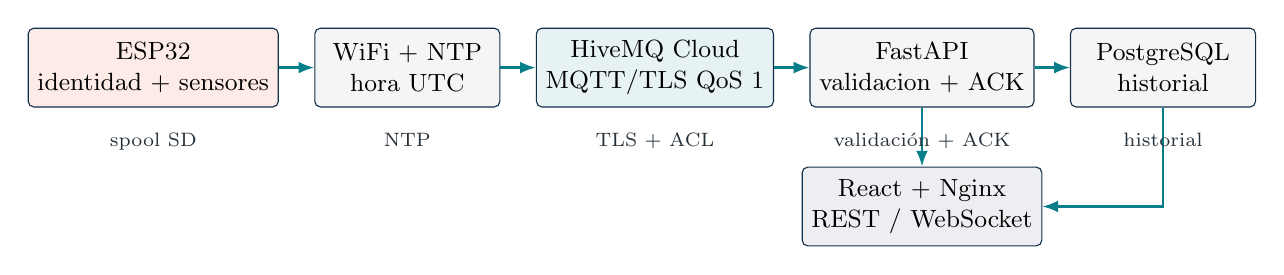
\begin{tikzpicture}[
  node distance=0.75cm and 0.45cm,
  box/.style={draw=navy, rounded corners=2pt, fill=softgray,
    minimum width=2.35cm, minimum height=1.0cm, align=center, font=\small},
  edge/.style={-{Latex[length=2mm]}, thick, draw=teal},
  note/.style={font=\scriptsize, align=center, text=ink}
]
\node[box, fill=orange!14] (esp) {ESP32\\identidad + sensores};
\node[box, right=of esp] (net) {WiFi + NTP\\hora UTC};
\node[box, right=of net, fill=teal!10] (broker) {HiveMQ Cloud\\MQTT/TLS QoS 1};
\node[box, right=of broker] (api) {FastAPI\\validacion + ACK};
\node[box, right=of api] (db) {PostgreSQL\\historial};
\node[box, below=of api, fill=navy!8] (web) {React + Nginx\\REST / WebSocket};
\draw[edge] (esp) -- (net);
\draw[edge] (net) -- (broker);
\draw[edge] (broker) -- (api);
\draw[edge] (api) -- (db);
\draw[edge] (db.south) |- (web.east);
\draw[edge] (api) -- (web);
\node[note, below=0.2cm of esp] {spool SD};
\node[note, below=0.2cm of net] {NTP};
\node[note, below=0.2cm of broker] {TLS + ACL};
\node[note, below=0.2cm of api] {validación + ACK};
\node[note, below=0.2cm of db] {historial};
\end{tikzpicture}
\caption{Flujo lógico de la integración validada. Las flechas representan
interfaces del sistema; no implican que cada periférico del ESP32 haya sido
conectado durante esta sesión.}
\label{fig:arquitectura}
\end{figure}

\section{Contratos y tópicos}

La versión integrada usa telemetría v3. Cada muestra conserva
\code{vehicle\_id}, \code{device\_id}, \code{boot\_id}, \code{sequence},
\code{sample\_id}, \code{time\_valid}, \code{replayed} y \code{simulated},
además de las banderas de validez de sensores. El backend agrega
\code{received\_at}, de modo que una hora de medición ausente no se reemplaza
por una fecha inventada.

Los tópicos canónicos de la identidad real son:

\begin{lstlisting}
vehiclesense/v1/vehicles/vehicle-001/devices/esp32-d0ef7645f640/telemetry
vehiclesense/v1/vehicles/vehicle-001/devices/esp32-d0ef7645f640/status
vehiclesense/v1/vehicles/vehicle-001/devices/esp32-d0ef7645f640/events
vehiclesense/v1/vehicles/vehicle-001/devices/esp32-d0ef7645f640/acoustic
vehiclesense/v1/vehicles/vehicle-001/devices/esp32-d0ef7645f640/commands
vehiclesense/v1/vehicles/vehicle-001/devices/esp32-d0ef7645f640/command-acks
\end{lstlisting}

El dispositivo publica telemetría, estado, eventos, acústica y acuses; solo se
suscribe a \code{commands}. El backend se suscribe a las ramas de entrada y
publica comandos. El estado \code{online} se publica retenido y el LWT
\code{offline} está implementado para una desconexión inesperada, pero la
transición LWT todavía no se indujo en la prueba física de este informe.

\section{Capas de validación}

Antes de la sesión física se mantuvieron las pruebas unitarias de payload,
contratos MQTT, colas offline, backend, frontend y simulador. En conjunto, la
matriz automatizada registrada en el estado del proyecto reportó 24/24 builds
ESP32, 34/34 casos Unity nativos, fixtures contractuales válidos e inválidos,
15/15 pruebas backend y 6/6 pruebas frontend. Estas cifras son una base de
software; la sesión descrita en los capítulos siguientes añade la dimensión
física.

\section{Lectura de identidad}

La identidad no se inventó a partir de la etiqueta de la placa. Se leyó el
registro eFuse del chip por el puerto serial USB-UART. El resultado identificó un
ESP32-D0WD-V3, revisión 3.1, con MAC de fábrica:

\begin{center}
\fbox{\Large\code{d0:ef:76:45:f6:40}}
\end{center}

La normalización elimina dos puntos y utiliza minúsculas para formar
\code{esp32-d0ef7645f640}. Esta regla es determinista y permite repetir el
registro para otra placa sin reutilizar la identidad del dispositivo anterior.
El vehículo se mantuvo separado de la identidad física y se asignó como
\code{vehicle-001}.

\paragraph{Ficha de identidad y transporte.}
\begin{itemize}[leftmargin=0pt,label={}]
  \item \textbf{Chip:} ESP32-D0WD-V3, revisión 3.1.
  \item \textbf{MAC eFuse:} \code{d0:ef:76:45:f6:40}.
  \item \textbf{\code{vehicle\_id}:} \code{vehicle-001}.
  \item \textbf{\code{device\_id}:} \code{esp32-d0ef7645f640}.
  \item \textbf{Firmware:} \code{0.2.0}, perfil \code{vehiclesense\_wifi}.
  \item \textbf{Broker:} HiveMQ Cloud, MQTT/TLS TCP, puerto 8883.
  \item \textbf{Credencial:} \code{esp32-d0ef7645f640}, exclusiva para el dispositivo.
  \item \textbf{ACL:} raíz MQTT del vehículo y dispositivo; sin permiso global \code{\#}.
\end{itemize}

\section{Registro en el backend}

Con el auto-registro deshabilitado, se crearon primero el vehículo y el
dispositivo mediante la API. Esta secuencia evita que un cliente que conozca un
nombre plausible pueda crear identidades espontáneas. El resultado observable
en PostgreSQL fue un vehículo y un dispositivo físico asociado. La API devolvió
posteriormente el mismo par de IDs, el estado \code{online}, firmware
\code{0.2.0}, una hora \code{last\_seen\_at} y la marca \code{simulated=false}.

\section{Credencial y ACL en HiveMQ}

Se creó una credencial propia para el ESP32, separada de la credencial del
backend. La permission se nombró
\code{esp32-d0ef7645f640-scope} y limita el acceso a:

\begin{lstlisting}
vehiclesense/v1/vehicles/vehicle-001/devices/esp32-d0ef7645f640/#
\end{lstlisting}

Esta raíz es una concesión acotada para el prototipo: permite las ramas de
telemetría, estado, eventos, acústica, comandos y acuses de una sola identidad,
pero no autoriza otros vehículos o dispositivos. La contraseña se probó en el
cliente local y no se imprimió en el monitor ni se guardó en Git. El backend
conserva otra credencial con sus permisos de suscripción y publicación.

\section{Configuración separada de secretos}

El archivo versionado \code{include/secrets\_example.h} solo contiene nombres
de variables y valores de ejemplo. El archivo activo \code{include/secrets.h}
está ignorado por Git y contiene la red WiFi del hotspot, la credencial HiveMQ y
las identidades reales. Esta separación permite compilar el proyecto sin
exponer contraseñas en el informe, capturas o commits.

\section{Puesta en marcha del firmware}

\section{Secuencia de arranque}

El perfil \code{vehiclesense\_wifi} ejecuta una secuencia deliberadamente
conservadora:

\begin{enumerate}
  \item inicializa la identidad y el registro serial;
  \item asocia la interfaz WiFi al hotspot configurado;
  \item solicita NTP y espera una hora UTC dentro del intervalo permitido;
  \item inicializa ESP-MQTT sobre TLS con la CA compilada;
  \item se suscribe a comandos, publica el estado retenido \code{online} y
        comienza la telemetría QoS 1;
  \item mantiene la adquisición local aunque un periférico esté ausente.
\end{enumerate}

La lógica no considera suficiente que WiFi esté conectado: el handshake TLS se
realiza después de disponer de una hora válida. Esto evita que el certificado
del broker sea rechazado por una fecha de 1970 o por una hora todavía no
sincronizada.

\section{Corrección del tiempo NTP}

La primera ejecución solicitaba NTP correctamente, pero la función de validación
comparaba el resultado con el límite \code{4102444800} usando un tipo que en el
entorno ESP32 coincidía con \code{time\_t} de 32 bits. El literal se convertía
de forma incorrecta y una fecha de 2026 se trataba como inválida. El cambio
adoptado fue mantener los límites como \code{int64\_t} y convertir el valor de
\code{time(nullptr)} antes de compararlo:

\begin{lstlisting}[language=C++]
constexpr int64_t kMinimumValidEpoch = 1704067200LL;
constexpr int64_t kMaximumValidEpoch = 4102444800LL;
const int64_t now = static_cast<int64_t>(time(nullptr));
return now >= kMinimumValidEpoch && now < kMaximumValidEpoch;
\end{lstlisting}

Después de la corrección, el monitor confirmó \code{time\_valid=true}. El
backend recibió \code{measured\_at} y conservó por separado
\code{received\_at}, como define el contrato.

\section{Corrección de la cadena TLS}

El segundo bloqueo apareció durante el handshake. El firmware referenciaba el
bundle de certificados de Arduino, pero ese bundle no estaba inicializado
en este perfil. El serial registró un fallo TLS con \code{error=32794} y
\code{stack=30336}. Desactivar la verificación no era una opción aceptable:
habría ocultado el problema y debilitado el transporte.

Se reemplazó la referencia por el ancla pública ISRG Root X1 en el archivo
\code{TrustedRootCa.h} de comunicación y se mantuvo activa la comprobación
del nombre del host. La biblioteca ESP-MQTT siguió
usando TLS TCP y el hostname del cluster. La raíz es material público de
confianza, no una llave privada; aun así, debe revisarse si HiveMQ cambia su
cadena de certificados.

\section{Corrección de credenciales}

Con el certificado resuelto, el broker todavía podía rechazar una sesión si la
contraseña local no correspondía a la credencial recién creada. Se comparó el
nombre de usuario configurado con el registro de HiveMQ, se actualizó el secreto
local y se observó un CONNACK MQTT de código cero en la prueba de diagnóstico.
El valor de la contraseña no se reprodujo en ningún log ni en este informe.

\section{Carga y monitor serial}

La imagen final compiló y se cargó por el adaptador USB-UART identificado como
\code{/dev/cu.usbserial-0001}. El perfil utilizó 24.1~\% de RAM y 58.1~\% de
flash reportados por PlatformIO. El arranque final correspondió al
\code{boot\_id=14}. La siguiente transcripción es un resumen de líneas
observadas; se omiten credenciales y datos de red no necesarios:

\begin{lstlisting}
boot_id=14
wifi_connected=true
time_valid=true
mqtt_connected=true
HiveMQ connected with TLS; command ACL requested
Telemetry PUBACK token=20
\end{lstlisting}

La asociación WiFi tardó más que el primer ciclo de diagnóstico y presentó un
estado transitorio \code{wifi\_connected=false} alrededor de los diez segundos.
No se interpretó ese estado intermedio como fallo definitivo porque el mismo
arranque alcanzó NTP, TLS y MQTT poco después.

\section{Muestras y respuesta del backend}

La consulta productiva de dispositivos devolvió un único registro físico. La
respuesta se conserva aquí como una ficha para que pueda compararse con una
ejecución posterior:

\begin{itemize}[leftmargin=0pt,label={}]
  \item \textbf{\code{device\_id}:} \code{esp32-d0ef7645f640}.
  \item \textbf{\code{vehicle\_id}:} \code{vehicle-001}.
  \item \textbf{\code{status}:} \code{online}.
  \item \textbf{\code{firmware\_version}:} \code{0.2.0}.
  \item \textbf{\code{simulated}:} \code{false}.
  \item \textbf{\code{last\_seen\_at}:} 2026-09-01T03:55:29.865949+00:00.
\end{itemize}

La consulta de telemetría con ventana de una hora y límite de veinte devolvió
veinte muestras recientes. La última identificada en esa consulta fue
\code{esp32-d0ef7645f640:13:275}, medida a las 03:55:26 UTC y recibida por el
backend a las 03:55:26.747851 UTC. El identificador conserva el boot y la
secuencia, lo que permite deduplicar una reentrega QoS 1.

\section{Cronología resumida}

\begin{figure}[htbp]
\centering
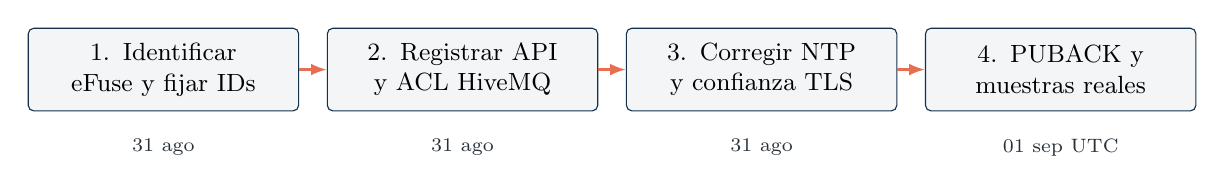
\begin{tikzpicture}[
  timelinebox/.style={draw=navy, rounded corners=2pt, fill=softgray,
    text width=3.2cm, minimum height=1.05cm, align=center, font=\small},
  arrow/.style={-{Latex[length=2mm]}, thick, draw=orange}
]
\node[timelinebox] (a) {1. Identificar\\eFuse y fijar IDs};
\node[timelinebox, right=0.35cm of a] (b) {2. Registrar API\\y ACL HiveMQ};
\node[timelinebox, right=0.35cm of b] (c) {3. Corregir NTP\\y confianza TLS};
\node[timelinebox, right=0.35cm of c] (d) {4. PUBACK y\\muestras reales};
\draw[arrow] (a) -- (b);
\draw[arrow] (b) -- (c);
\draw[arrow] (c) -- (d);
\node[font=\scriptsize, text=ink, below=0.23cm of a] {31 ago};
\node[font=\scriptsize, text=ink, below=0.23cm of b] {31 ago};
\node[font=\scriptsize, text=ink, below=0.23cm of c] {31 ago};
\node[font=\scriptsize, text=ink, below=0.23cm of d] {01 sep UTC};
\end{tikzpicture}
\caption{Secuencia de resolución de bloqueos y aceptación del transporte.}
\label{fig:timeline}
\end{figure}

\clearpage
\section{Conclusiones}

Este tercer avance transforma la integración E2E de una hipótesis de software
en una observación física acotada. El ESP32 real fue identificado, registrado y
autenticado con una ACL individual. La corrección del tiempo NTP y de la cadena
de confianza TLS eliminó los dos bloqueos que impedían llegar al broker; la
corrección de la contraseña permitió completar el CONNACK. La secuencia final
mostró WiFi, hora válida, TLS, MQTT y PUBACK, y la API productiva devolvió el
dispositivo en línea y veinte muestras asociadas a los IDs correctos.

El resultado es suficiente para continuar con la línea base física de sensores,
fallos, replay y comandos. No es suficiente para afirmar que la PCB está lista,
que el sistema es tolerante a fallos, que los datos acústicos están calibrados o
que el proyecto constituye un sistema de seguridad vehicular. Mantener esas
fronteras explícitas permite que los siguientes informes se apoyen en evidencia
fechada y no en capturas o suposiciones.

\end{document}
